\documentclass[a4paper,14pt]{extarticle}

\usepackage{geometry}
\geometry{a4paper,tmargin=2cm,bmargin=2cm,lmargin=3cm,rmargin=1cm}
\usepackage[T2A]{fontenc}
\usepackage[utf8]{inputenc}
\usepackage[english,main=russian]{babel}
\usepackage{indentfirst}
\usepackage{graphicx}
\graphicspath{{./images/}}
\usepackage{setspace}
\linespread{1.3}
\usepackage{tempora}
\usepackage{amsmath}
\usepackage{booktabs}
\usepackage{array}
\usepackage{caption}
\usepackage{hyperref}
\hypersetup{unicode=true,hidelinks}
\usepackage{listings}

\sloppy
\clubpenalty=10000
\widowpenalty=10000



\lstset{basicstyle=\ttfamily\small,breaklines=true,
  columns=fullflexible,frame=single,numbers=none,
  showstringspaces=false,tabsize=4,captionpos=t,keepspaces=true}
\renewcommand{\lstlistingname}{Листинг}
\begin{document}

\begin{titlepage}
\thispagestyle{empty}

\vspace*{-60pt}

\hspace*{-82pt}
\begin{minipage}{0.3\textwidth}
\centering
\IfFileExists{images/emblem.png}{%
  
\includegraphics[width=0.9\textwidth]{emblem.png}%
}{%
  \IfFileExists{images/emblem.jpg}{%
    \includegraphics[width=0.9\textwidth]{emblem.jpg}%
  }{}%
}
\end{minipage}
\begin{minipage}{0.67\textwidth}
\small
\textbf{
\vspace*{-0.7ex}
\centerline{Министерство науки и высшего образования Российской Федерации}
\vspace*{-0.7ex}
\centerline{Федеральное государственное бюджетное образовательное учреждение}
\vspace*{-0.7ex}
\centerline{высшего образования}
\vspace*{-0.7ex}
\centerline{<<Московский государственный технический университет}
\vspace*{-0.7ex}
\centerline{имени Н. Э. Баумана}
\vspace*{-0.7ex}
\centerline{(национальный исследовательский университет)>>}
\vspace*{-0.7ex}
\centerline{(МГТУ им. Н. Э. Баумана)}
}
\end{minipage}

\vspace{-25pt}
\hspace{-35pt}\rule{\textwidth}{2.3pt}

\vspace*{-20.3pt}
\hspace{-35pt}\rule{\textwidth}{0.4pt}

\vspace{1.5ex}
\hspace{-35pt}\noindent\small
ФАКУЛЬТЕТ\hspace{80pt} <<Информатика и системы управления>>

\vspace*{-16pt}
\hspace{47pt}\rule{0.83\textwidth}{0.4pt}

\vspace{0.5ex}
\hspace{-35pt}\noindent\small
КАФЕДРА\hspace{50pt} <<Теоретическая информатика и компьютерные технологии>>

\vspace*{-16pt}
\hspace{30pt}\rule{0.866\textwidth}{0.4pt}

\vspace{11em}

\begin{center}
\Large \textbf{Лабораторная работа №3} \\
\large \textbf{по курсу <<Параллельные и распределённые системы>>} \\
\large <<Задача об обедающих философах>>
\end{center}

\normalsize

\vspace{8em}

\begin{flushright}
Студент группы ИУ9-51Б \\
Шалимов Д. И. \\
\vspace{2ex}
Преподаватель Царев А.С.
\end{flushright}

\bigskip
\vfill

\begin{center}
\textsl{Москва 2026}
\end{center}
\end{titlepage}

\setcounter{page}{2}
\tableofcontents
\newpage



\section{Постановка задачи}
Цель работы --- реализовать многопоточную модель задачи об обедающих
философах и исследовать доступ потоков к общим ресурсам.
За круглым столом находятся $N$ философов и $N$ вилок. Каждый философ
чередует размышление и еду; для еды нужны обе соседние вилки.
Одной вилкой одновременно может владеть только один участник.

Модель написана на Python: философу соответствует
\texttt{threading.Thread}, вилке --- \texttt{threading.Lock}.
У философа $i$ соседние вилки имеют номера $i$ и $(i+1)\bmod N$.
В коде нумерация начинается с нуля, в журнале и на рисунках --- с единицы.

\section{Реализация и синхронизация}
Все потоки выполняют один метод \texttt{philosopher} объекта \texttt{Table}.
Каждый сначала берёт соседнюю вилку с меньшим номером, затем --- с большим.
Для последнего философа это означает захват правой вилки раньше левой.
Ключевой фрагмент задаёт одинаковое правило для всех участников:

\begin{lstlisting}[language=Python,caption={Порядок захвата вилок}]
left, right = i, (i + 1) % self.count
order = sorted([(left, LEFT), (right, RIGHT)])
for fork, state in order:
    if not self.take(i, fork, state, rng):
        return
\end{lstlisting}

При таком порядке поток, удерживающий первую вилку, ждёт только ресурс
с большим номером. Замкнутая цепочка ожиданий потребовала бы строгого
возрастания номеров по кругу, что невозможно. Следовательно,
взаимоблокировка исключена. Несоседние философы могут есть одновременно;
их число не превышает $\lfloor N/2\rfloor$.
Строгая гарантия отсутствия голодания не заявляется: блокировки не
обеспечивают обязательного обслуживания в порядке прихода.

Времена размышления, взятия каждой вилки, еды и возвращения вилок
случайно выбираются из интервалов 0.10--0.25, 0.02--0.05,
0.10--0.20 и 0.02--0.05~с соответственно.
Вилки захватываются по отдельности. Состояние взятия включает ожидание
блокировки; во время задержки возвращения обе вилки ещё удерживаются,
а затем освобождаются подряд.

Общий старт организован через \texttt{Barrier} и событие \texttt{start}.
Событие \texttt{stop}, прерываемые задержки и тайм-аут
\texttt{acquire(timeout=0.01)} позволяют остановить потоки по времени.
Освобождение вилок в \texttt{finally} и ожидание всех потоков через
\texttt{join} обеспечивают корректное завершение.

Короткая блокировка \texttt{journal\_lock} защищает журнал, но не
удерживается во время размышления, еды или ожидания вилок.
Записываются пять состояний: размышление, взятие левой вилки,
взятие правой вилки, еда и возвращение вилок.
Запись на конечной границе времени закрывает интервал наблюдения,
а не обозначает новое действие.

\section{Результаты и анализ}
Рассмотрены два сохранённых запуска длительностью 10~с, при $N=5$ и
$N=9$, с \texttt{seed=1}. Фиксированный seed задаёт последовательности
случайных задержек, но не расписание потоков, поэтому повторный запуск
может дать другие счётчики.

\begin{table}[htbp]\centering
\caption{Результаты моделирования}
\small
\begin{tabular}{r l r}
\toprule
$N$ & Приёмов пищи по философам & Максимум едящих \\
\midrule
5 & 15, 15, 15, 15, 15 & 2 \\
9 & 15, 15, 15, 16, 15, 16, 16, 17, 15 & 4 \\
\bottomrule
\end{tabular}
\end{table}

Время с завершением потоков составило 10.010~с и 10.013~с соответственно.
Проверка сохранённых журналов не обнаружила одновременной еды соседей,
владения одной вилкой разными философами или еды без двух соседних вилок.
Максимальное число одновременно едящих совпало с границей
$\lfloor N/2\rfloor$ в обоих запусках.
Диаграммы на рисунке~\ref{fig:timelines} показывают чередование состояний
и одновременную еду несоседних участников.

\begin{figure}[htbp]\centering
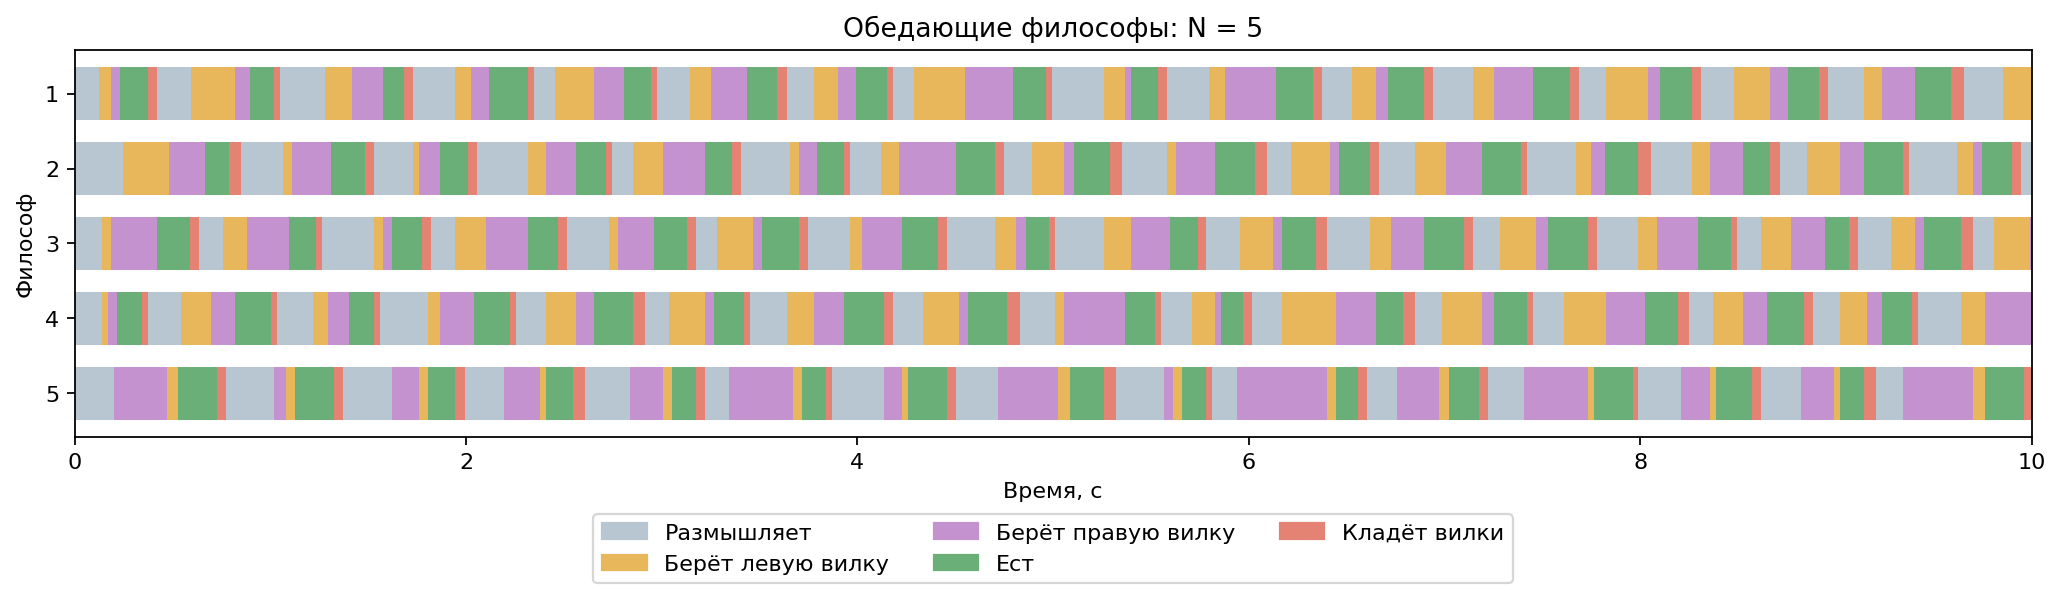
\includegraphics[width=\textwidth]{lab3_n5_timeline.png}\par\medskip
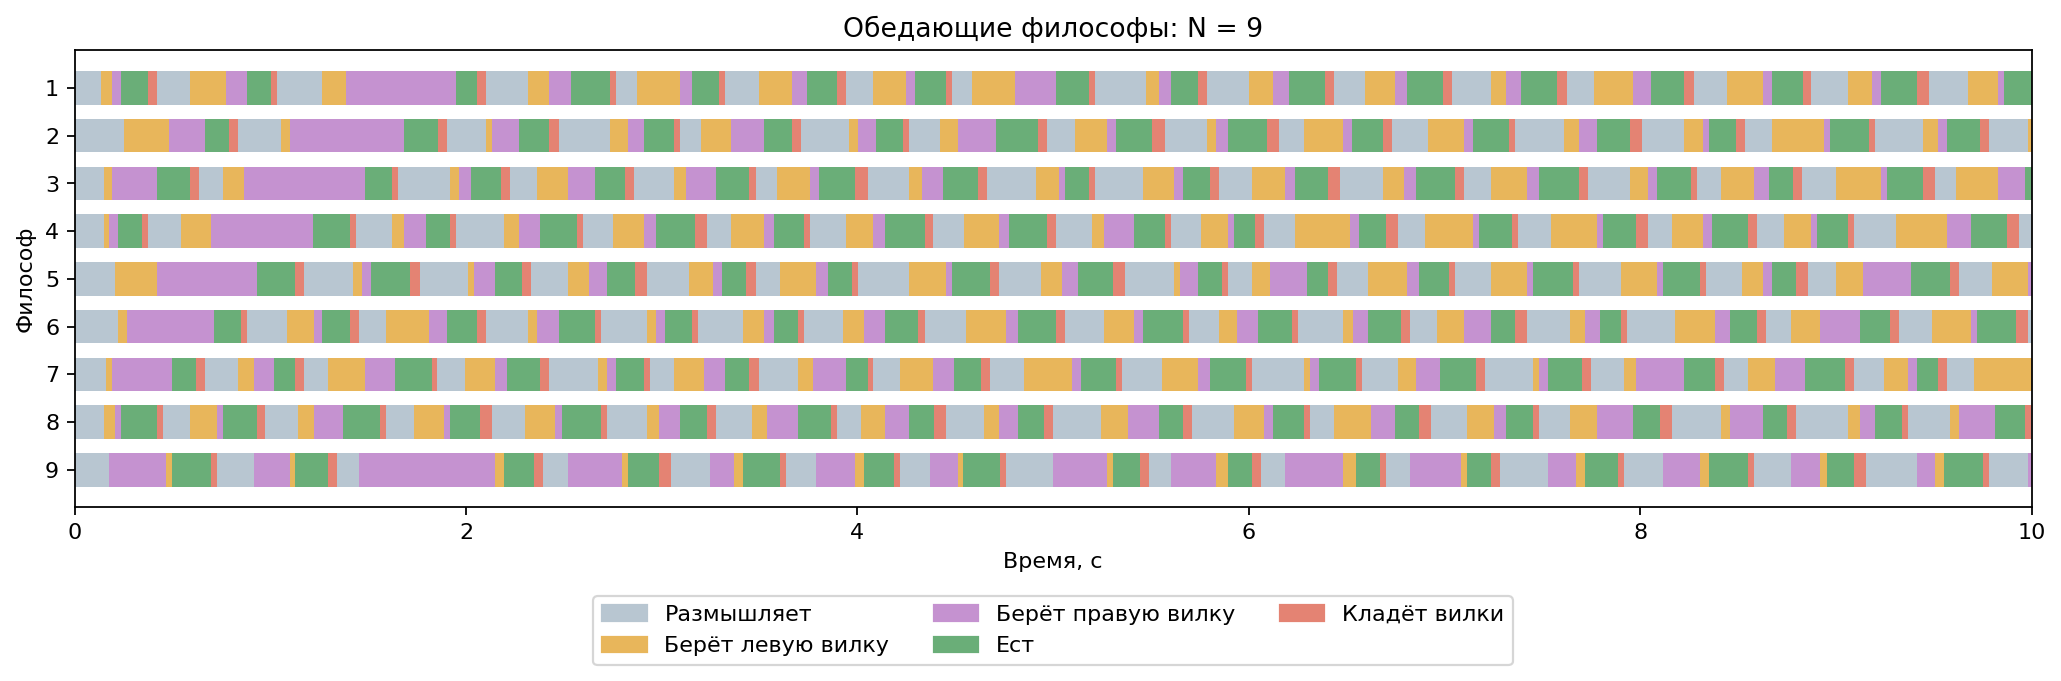
\includegraphics[width=\textwidth]{lab3_n9_timeline.png}
\caption{Временные диаграммы для пяти и девяти философов}
\label{fig:timelines}
\end{figure}

Каждый философ завершил не менее 15 приёмов пищи. При $N=9$ счётчики
различаются из-за конкуренции за вилки и порядка работы потоков.
Отсутствие голодания в этих запусках является наблюдением,
а не общей гарантией алгоритма.

\section{Вывод}
Построена многопоточная модель с отдельными блокировками общих ресурсов.
Упорядоченный захват вилок исключает взаимоблокировку и сохраняет
возможность одновременной еды несоседних философов.
Журналы и диаграммы подтверждают соблюдение ограничений в сохранённых
экспериментах. Событие остановки и освобождение ресурсов в
\texttt{finally} позволяют завершить модель по заданному времени.

\end{document}
